\vspace{0.5cm}


\section*{Problema 5.2}
El área del rayo paralelo entre las latitudes mencionadas es $2a\cos{\varphi} *a\dd{\varphi} \cos{\varphi}$, mientras que el área de la superficie terrestre entre las latitudes dadas es $2\pi a\cos{\varphi} *a\dd{\varphi}$. Entonces, se tiene
	$$ F = \frac{2a\cos{\varphi} *a\dd{\varphi} \cos{\varphi}}{2\pi a\cos{\varphi} *a\dd{\varphi}} S_o = \frac{S_o}{\pi} \cos{\varphi}. $$
	\begin{enumerate}[a)]
		\item Por lo visto en el capitulo dos, se tiene el balance en el tope y en la superficie de la atmosfera
			$$ A\uparrow = \sigma T_a ^4 = (1 - \alpha _p) \frac{S_o}{\pi} \cos{\varphi}, $$
			$$ \sigma T_s ^4 = A\downarrow + (1 - \alpha _p) \frac{S_o}{\pi} \cos{\varphi}. $$
		Además, se sabe que $A\uparrow = A\downarrow$, por lo que
			$$ 2(1 - \alpha _p) \frac{S_o}{\pi} \cos{\varphi} = \sigma T_s ^4, $$
			$$ T_s = \qty(\frac{8\cos{\varphi}}{\pi})^{\frac{1}{4}} \qty(\frac{(1 - \alpha _p) S_o}{4\sigma})^{\frac{1}{4}}. $$
		\item Con $T_e = 255K$, para las latitudes dadas se valúa lo encontrado el inciso anterior
			$$ T_s (0^o) = \qty(\frac{8\cos{0}}{\pi})^{\frac{1}{4}} 255K = 322.13K, $$
			$$ T_s (30^o) = \qty(\frac{8\cos{30}}{\pi})^{\frac{1}{4}} 255K = 310.75K, $$
			$$ T_s (60^o) = \qty(\frac{8\cos{60}}{\pi})^{\frac{1}{4}} 255K = 270.87K. $$
	\end{enumerate}
	
\section*{Problema 5.3}
Tomando el balance hidrostático y la ley de gas ideal se tiene
	$$ \pdv{z}{p} = - \frac{RT}{gp}, $$
entonces, podemos integrar, esta dependerá de la presión en la superficie
	$$ z(p) = \frac{R}{g} \int _p ^{p_s} T \underbrace{\frac{\dd{p}}{p}}_{\dd{\ln{p}}} = \frac{R}{g} \int _p ^{p_s} T \dd{\ln{p}} \quad \Rightarrow \quad z(p) = \frac{R}{g} \expval{T} \int _p ^{p_s} \dd{\ln{p}}. $$
Ahora, para $\Delta z = z(500hPa) - z(1000hPa)$, integrando
	$$ \Delta z = \frac{R \expval{T}}{g} \ln{2}. $$
	
	
\begin{enumerate}[a)]
	\item Tomando las temperaturas del problema anterior, encontramos el grosor valuando la expresión encontrada
		$$ \Delta z (\text{a } 30^o) = 6301.6 $$
		$$ \Delta z (\text{a } 60^o) = 5947.4. $$
	\item 
\end{enumerate}



%\section*{Anexo}
%\begin{figure}[H]
%	\centering
%	 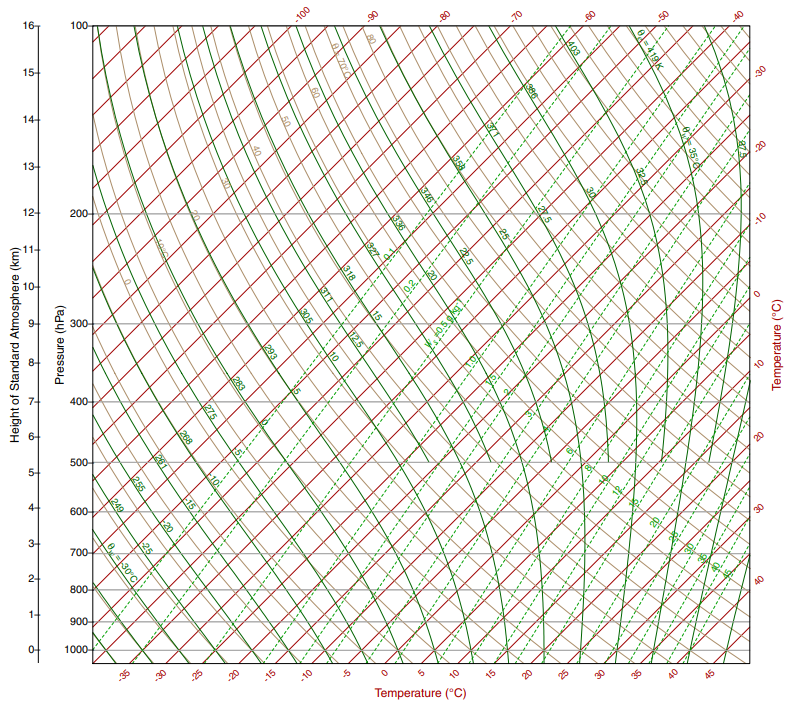
\includegraphics[scale=0.7]{./img/skewTlnp.png}
%	 \caption{Skew $T-\ln{p}$ Chart, book website.}
%	 \label{skew}
%\end{figure}



















%%%%%